O objetivo das maquinas de vetores de suporte é encontrar um hipeplano em um espaço n-dimensional que consiga separar os pontos de categorias distintas. Um exemplo visual da separação de duas categorias utilizando  hiperplanos é mostrado na figura \ref{hiperplanes}

\begin{figure}[h]
\centering
\caption{Hiperplanos nos espaços 2D e 3D}
  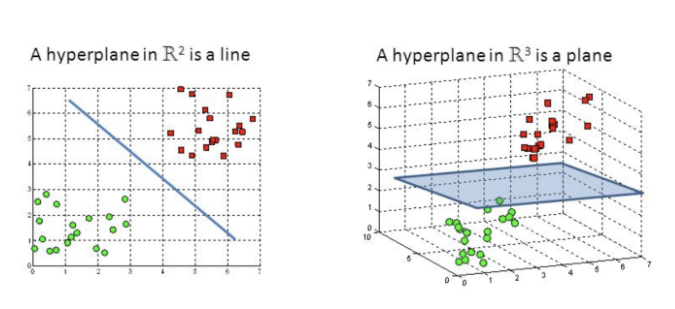
\includegraphics[width=8cm]{"images/hiperplaneExample.png"}
  \centering
\caption*{Fonte: }%%"https://machine-learning-and-data-science-with-python.readthedocs.io/en/latest/assignment5_sup_ml.html"}
\label{fig: hiperplanes}
\end{figure} 

